\documentclass{beamer}
%% Possible paper sizes: a0, a0b, a1, a2, a3, a4.
%% Possible orientations: portrait, landscape
%% Font sizes can be changed using the scale option.
%% Universidade de São Paulo
%% IME
%% Instituto de Matemática e Estatística
\usepackage[size=a1,orientation=portrait,scale=1.8]{beamerposter}

\usepackage[utf8]{inputenc}
\usepackage[T1]{fontenc}
\usepackage{libertine}
\usepackage[scaled=0.92]{inconsolata}
\usepackage[libertine]{newtxmath}
\usepackage{ragged2e}
\usepackage[sort,numbers]{natbib}
\usepackage[latin1]{inputenc}
\usepackage{caption}
\captionsetup[figure]{font=small}

\beamertemplatenavigationsymbolsempty

\definecolor{RedD}         {RGB}{215, 0, 0} 
\setbeamercolor{block title}{fg=RedD,bg=white}
\setbeamercolor{block body}{fg=black,bg=white}
\setbeamercolor{local structure}{fg=RedD}
\setbeamercolor{bibliography structure}{fg=RedD}
\setbeamercolor{bibliography item}{fg=black,bg=white}
\setbeamercolor{bibliography entry author}{fg=black,bg=white}
\setbeamercolor{bibliography item}{fg=black,bg=white}
\setbeamercolor{bibliography entry location}{fg=black} 
\setbeamercolor{bibliography entry note}{fg=black} 


\author[giuliano.belinassi@usp.br]{Giuliano Augusto Faulin Belinassi}
\title{Optimizing a Boundary Elements Method for Stationary Elastodynamic Problems Implementation with GPUs}
\institute{Instituto de Matemática e Estatística - Universidade de São Paulo}
%\subtitle{Evaluating Scalability for \\Complex Event Processing \\in the Context of Smart Cities}
%\advisor{Advisor: Kelly Rosa Braghetto}
%\abstract{ffs@ime.usp.br}

%$\citenum{belinassi:2017}$ $\citenum{carrion:02}$ $\citenum{katsikadelis:2016}$

\addtobeamertemplate{headline}{} {
 \leavevmode
  \begin{columns}[T]
    \begin{column}{.15\linewidth}
        \vskip2.5cm
        \hskip1cm
        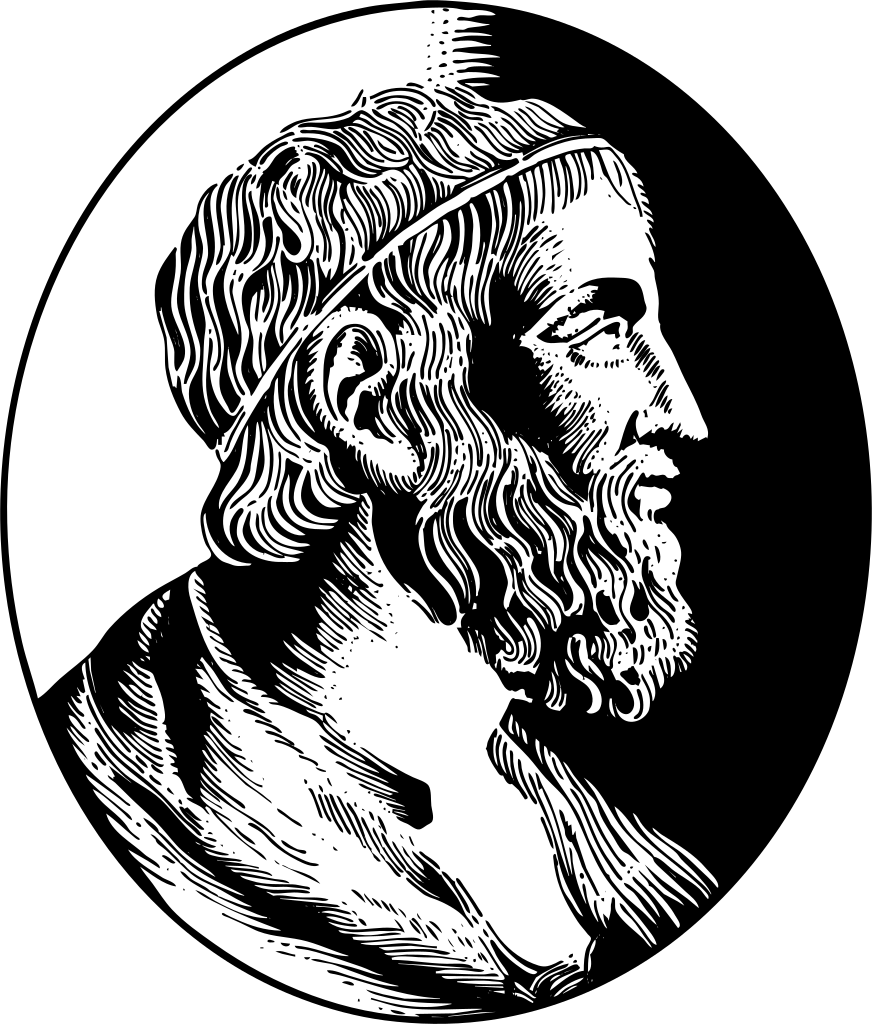
\includegraphics[width=1.1\linewidth]{IMElogo.png}
    \end{column}
    \begin{column}{.7\linewidth}
         \vskip2cm
         \centering
         \usebeamercolor{title in headline}{\color{black}\Huge{\textbf{\inserttitle}}\\[0.5ex]}
         \vskip.5cm
%         \usebeamercolor{subtitle in headline}{\color{black}\huge{\insertsubtitle}\\[0.5ex]}
         \vskip.5cm
         \usebeamercolor{author in headline}{\color{fg}\Large{\textbf{\insertauthor}}\\[1ex]}
         \usebeamercolor{}{\color{fg}\Large{\textbf{Supervisor: Alfredo Goldman \\Co-supervisor: Marco D. Gubitoso}}\\[0.5ex]}
         \usebeamercolor{institute in headline}{\color{fg}\large{\insertinstitute}\\[1ex]}
         \usebeamercolor{email in headline}{\color{fg}\large{\url{giuliano.belinassi@usp.br}}\\[0.5ex]}
         \vskip1cm
    \end{column}
    \begin{column}{.15\linewidth}
    	\vskip 2.1cm
        \begin{flushleft}
        
\includegraphics[width=\linewidth]{USP.jpg}
        \end{flushleft}
        \hskip1cm
        
    \end{column}        
   \vspace{1cm}
  \end{columns}
 \vspace{0.5in}
 \hspace{0.5in}\begin{beamercolorbox}[wd=47in,colsep=0.15cm]{black}\end{beamercolorbox}
 \vspace{-1.5in}
}
\begin{document}
\begin{frame}[fragile]\centering

\begin{columns}[T]

%%%% First Column
\begin{column}{.46\textwidth}

\begin{block}{Introduction}\justifying

\begin{itemize}

\item The Boundary Element Method (BEM) is a very efficient alternative for modeling unlimited domains.
\item This method can be used for numerically modeling the stationary behavior of 3D wave propagation in the soil. [$\citenum{katsikadelis:2016}$]
\item It can be used for analyzing the vibration created by heavy machines, railway lines, or earthquakes.

\end{itemize}

\vspace{0.5cm}

\begin{figure}
	\centering
	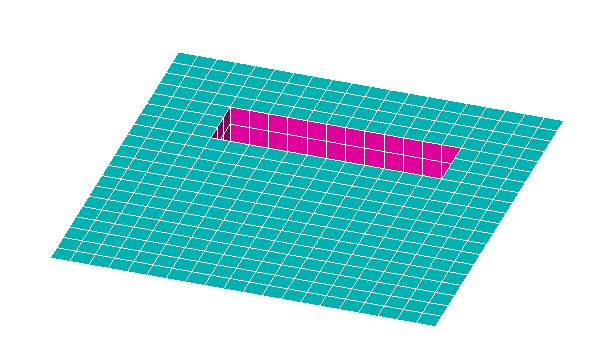
\includegraphics[scale=0.7]{trincheira.png}
	\caption{Example of a surface.}

\end{figure}

\end{block}

\begin{block}{BEM Formulation Background}\justifying

\begin{itemize}
\item Boundary Integral Equation for Stationary Elastodynamic Problems [$\citenum{carrion:02}$]:
\begin{equation}
\begin{split}
	c_{ij}u_{j}(\xi,\omega) + \int_S t_{ij}^*(\xi, x, \omega)u_j (x, \omega)\text{d}S(x) = \\
	= \int_S u_{ij}^*(\xi, x, \omega) t_j(x, \omega)\text{d}S(x) \label{bem_formulation} \nonumber
\end{split}
\end{equation}

\item After performing the geometry discretization, above equation can be represented in matrix form as $Hu = Gt$.
\item Numerically, these integrals can be computed using the Gaussian quadrature.

\end{itemize}
\end{block}

\begin{block}{Objectives}\justifying
\begin{itemize}

\item Bring a legacy implementation of BEM for Estationary Elastodynamics Problems to a contemporary computing scenario, enabling the usage of multicore processors and GPUs.
\item Accelerate the overall performance to simulate surfaces with a higher number of mesh elements

\end{itemize}
\end{block}

\end{column}

%%%% Second Column
\begin{column}{.46\textwidth}



\begin{block}{Results}

We applied the paralelization approach described in [$\citenum{belinassi:2017}$] together with MAGMA's LU decomposition. 

\begin{figure}
	\centering
	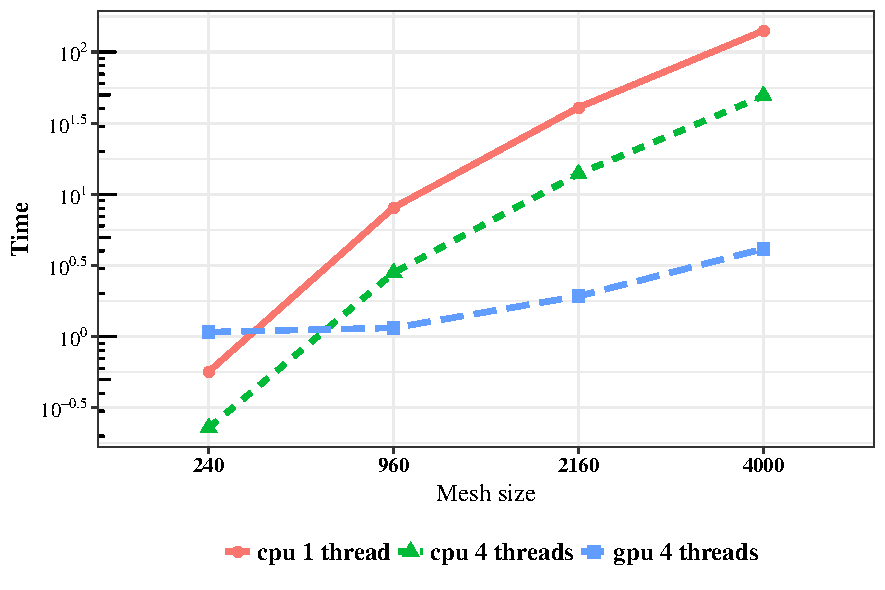
\includegraphics[scale=1.4]{venus_total.pdf}
	\caption{Total elapsed time in a \texttt{AMD A10-7700K} paired with a \texttt{GeForce GTX 980}}
	\label{fig:venus}
\end{figure}

\begin{figure}[ht]
	\centering
	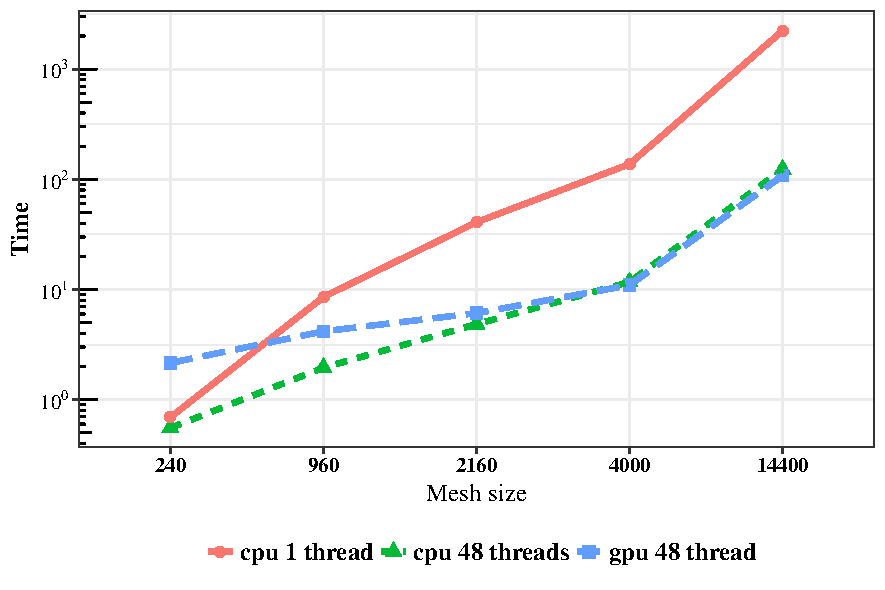
\includegraphics[scale=1.4]{total_brucutuiv.pdf}
	\caption{Total elapsed time in a \texttt{$2\times$ Xeon E6-2650 v4} paired with a \texttt{Tesla K40}}
	\label{fig:total_brucutuiv}
	\label{fig:brucutuiv}
\end{figure}

\end{block}

\begin{block}{Conclusions}\justifying
\begin{itemize}

%\item GPUs can be used to accelerate the overall application's performance.
\item Better speedups can be obtained if a load balancer is implemented. The current implementation does not use both CPU and GPU simultaneously.


\end{itemize}
\end{block}


\begin{block}{References}
%\bibliographystyle{plainnat}
\bibliographystyle{unsrtnat}
{\footnotesize
\bibliography{ref.bib}}
%\bibliography{ref.bib}
%\bibliographystyle{sbc}
%\bibliography{ref.bib}
\end{block}

\end{column}
\end{columns}

%\begin{block}{Proposal}
%\begin{itemize}
%\item Search all scalability technics for Complex Event Processing and find which ones can be combined to lower resource usage.
%\item Monitor the CPU, memory and bandwidth usage to more easily adapt to the addition or subtraction of available machines for processing
%\item Discover Smart Cities requirements that may affect the  Scalability of the CEP system and try to overcome them.
%\item Maybe use the city natural disposition and features to improve the processing, based on the correlation between geographical localization and information relevance to people on that place.
%\end{itemize}
%\end{block}
%\begin{columns}[T]
%\begin{column}{.9\linewidth}
%\begin{block}{}
%This Research is funded by CAPES \\(Coordenação de Aperfeiçoamento de Pessoal de Nível Superior) 
%\end{block}
%\end{column}
%\begin{column}{.1\linewidth}
%
\includegraphics[height=5cm,width=5cm]{capes.jpg}
%\end{column}
%\end{columns}
\end{frame}
\end{document}
